\subsection{Measurement methods}
We can measure the emission spectrum pretty easily (the whole apparatus is already set up): Just place the metal plates onto their designated spot in the X-ray beam, close the chamber door and start the X-ray radiation by pressing one button. The results are displayed on the computer after setting up the CassyLab programm.  

The metal probes, see \cref{fig:Metalplates.jpeg}, are examined by recording the counts for 3 minutes. After calibrating with iron and Molybdenum, the channels and their counts are displayed with the correct energy, now gaussian curves can be fitted to he \(K_\alpha,\,K_\beta\) peaks. 
\xfigure{htbp}{width=0.6\textwidth}{Metalplates.jpeg}{metal probes and alloys}{right side: used metal probes; left side: unknown alloys}

The programm allows to insert the theoretical/literature energy values/emission lines of different elements into the graph. This feature is used to roughly fit an elements characteristic lines to the peaks in the spectrum of unknown alloys, resulting in an approximation of the alloys' composition. An example is shown in \cref{fig:unknownalloy}.
\vfill
\subsection{Lab protocol / data sheet}
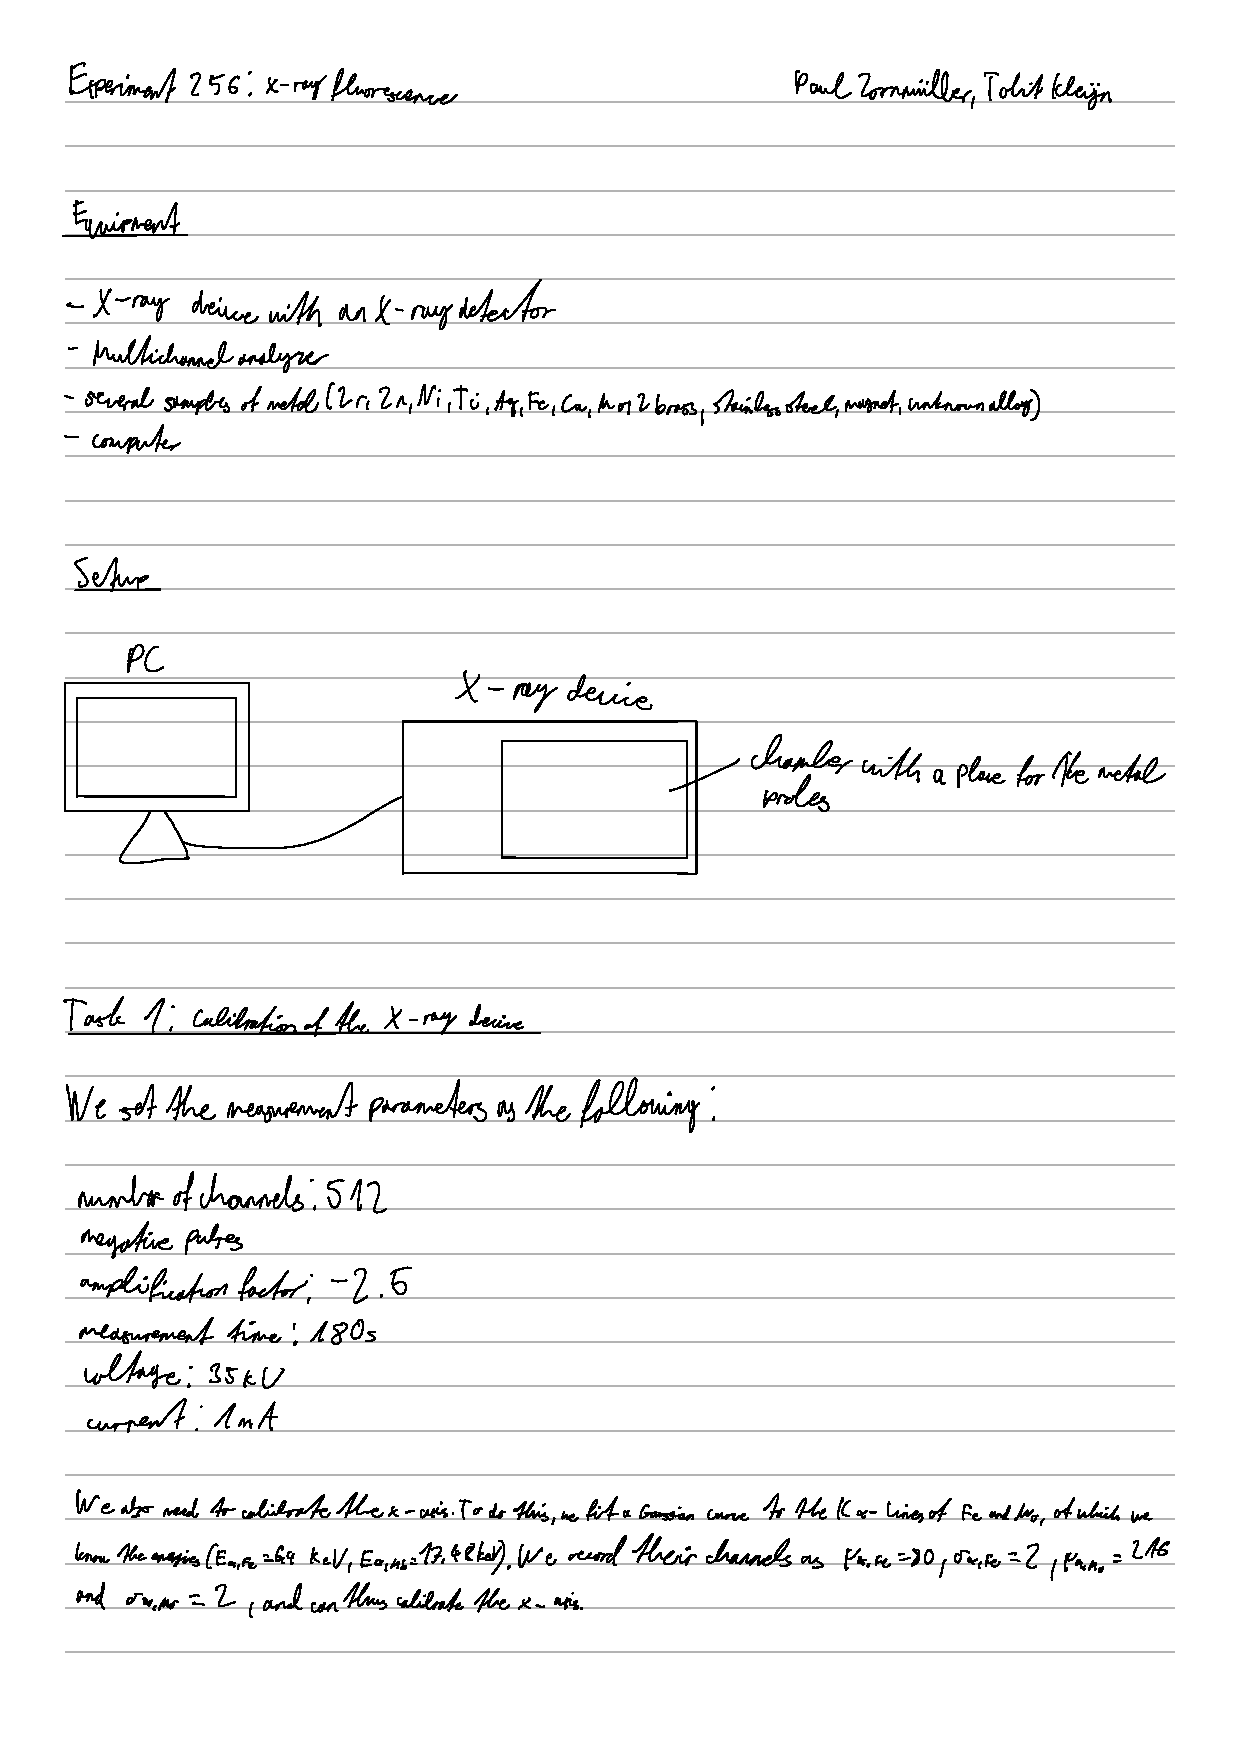
\includepdf[pages=-]{./images/Messprotokoll_256}
